\usetikzlibrary{automata, positioning}
\smalltitle{سوال 3}
\begin{enumerate}
  \item \phantom{text}
  \begin{latin}
    \noindent
    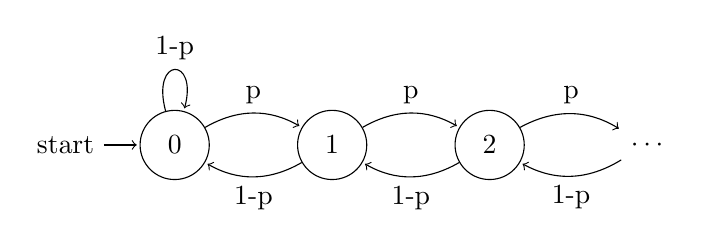
\begin{tikzpicture}[shorten >=1pt, node distance=2cm, on grid, auto]
     \node[state, initial] (q0) {$0$};
     \node[state] (q1) [right=of q0] {$1$};
     \node[state] (q2) [right=of q1] {$2$};
     \node (dots) [right=of q2] {$\cdots$};
  
     \path[->]
     (q0) edge [bend left] node {p} (q1)
     (q1) edge [bend left] node {p} (q2)
     (q1) edge [bend left] node {1-p} (q0)
     (q2) edge [bend left] node {1-p} (q1)
     (q2) edge [bend left] node {p} (dots)
     (dots) edge [bend left] node {1-p} (q2)
     (q0) edge [loop above] node {1-p} ();
  \end{tikzpicture}
 \end{latin}
 \item \phantom{text}
  \begin{latin}
    \noindent
    Lets write our probabilities according to $\pi_0$\\\\
    $\pi_0 = (1-p)\pi_0 + (1-p)\pi_1 \rightarrow \pi_1 \Rightarrow \pi_1 = \frac{p}{1-p}*\pi_0$ \\\\
    $\pi_1 = (p)\pi_0 + (1-p)\pi_2 \rightarrow (1-p)\pi_2 \Rightarrow \pi_2  = \frac{p}{1-p}*\pi_0 - p\pi_0=\frac{p^2}{(1-p)^2}*\pi_0$ \\\\
    $\pi_2 = (p)\pi_1 + (1-p)\pi_3 \rightarrow (1-p)\pi_3 \Rightarrow \pi_3  = (\frac{p}{1-p})^2*\pi_0 - p\pi_1=\frac{p^3}{(1-p)^3}*\pi_0$ \\\\
    \vdots \\\\
    $\pi_{i-1} = (p)\pi_{i-2} + (1-p)\pi_{i} \rightarrow (1-p)\pi_{i} \Rightarrow \pi_i = (\frac{p}{1-p})^{i-1}*\pi_0 - p\pi_{i-1}=\frac{p^i}{(1-p)^{i}}*\pi_0$ \\\\
    $\pi_0 + \pi_1 + \pi_2 + \cdots + \pi_i + \cdots +\pi_n = 1 \rightarrow (1 + \frac{p}{1-p} + (\frac{p}{1-p})^2+\cdots+(\frac{p}{1-p})^n)\pi_0 = 1$ \\\\
    $\frac{p}{1-p} = a \rightarrow a^0 + a^1 + \cdots + a^n = \frac{a^n-1}{a-1}\xrightarrow[]{n \rightarrow \inf} = \frac{1}{1-a}\rightarrow \frac{1}{1-a}\pi_0=1\rightarrow\pi_0 = 1 - a = 1 - \frac{p}{1-p}$\\\\
    $\pi_i = (\frac{p}{1-p})^i * (1 - \frac{p}{1-p})$
  
 \end{latin}
 \item \phantom{text}
  \begin{latin}
    \noindent
    We know that : $0\leq\pi_i\leq1$\\\\
    $\pi_i = (\frac{p}{1-p})^i * (1 - \frac{p}{1-p})\xrightarrow[]{0 \leq i} 0 \leq 1 - \frac{p}{1-p} \leq 1$ \\\\
    We know that with probability 1, we go to state 0, because its the starting state : \\\\
    $0 < 1 - \frac{p}{1-p} \rightarrow 2p < 1 \rightarrow p < \frac{1}{2}$
  
 \end{latin}
\end{enumerate}
